\documentclass[10pt]{article}
\usepackage[a4paper,margin=16mm]{geometry}
\usepackage{mathptmx,amsmath,graphicx,booktabs,hyperref}
\setlength{\parindent}{0pt}\setlength{\parskip}{5pt}
\begin{document}
\begin{center}{\Large Actual F13 twist transfer and finite useful S3 comparisons}\\[5pt]
Quadratic-twist study, PR2381; cm8-transfer-20261025;25 October2026\end{center}
\textbf{Executed.} C++ and independent Rust verify all14 rational source points,
196 addition pairs, the exact two-point kernel, seven scalar images and72
separate main-source recoveries across12 base arms. No point map is constructed
by a scalar lookup. All source scalars verify; labels remain outside recovery.

\section*{An actual reduction on the order-seven subgroup}
Registered E/F13 has $y^2=x^3+x+4$, intermediate H has $y^2=x^3+4x+7$,
and the d2 monic twist T has $y^2=x^3+4x+6$. The translated degree-two
coordinate construction followed by unit5 scaling is
\[
 X=12(x+2/(x-10)),\qquad Y=8y(1-2/(x-10)^2).
\]
Infinity and kernel point(10,0) map to infinity. All other source denominators
are nonzero. Public lexicographic generator P=(0,2) maps to U=(8,11), both
order7. Lean constructs actual nonsingular elliptic points and kernel-checks
all subgroup scalar/addition identities. For Q in the selected source subgroup,
$\Phi(Q)=nU$ iff $Q=nP$, for every $n\in\mathrm{Fin}\,7$.
\begin{center}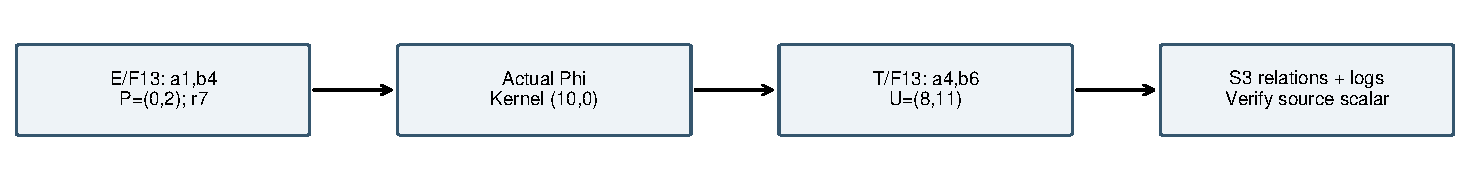
\includegraphics[width=\linewidth]{bridge.pdf}\end{center}
No unit c satisfies $c^4=4,c^6=8$. Lean also checks the necessary coefficient
equations for every admissible short-Weierstrass change with parameters u,r,s,t.
The general library classification/normalization bridge and generic geometric
isogeny theorem are not formalized by these finite checks. Exact ICV1 model
identities are retained; selected EC1 generator representations are not added.

\section*{Useful rows and named solver degree}
All three size-two bases per curve, all nine canonical pairings and all six
nonzero source targets remain:54 paired target comparisons. Transported and
pulled-back controls give12 arms,144 original/reduced complete certificates.
Every promoted row retains its witness in the three supplied input polynomials.

\begin{center}\begin{tabular}{lrr}\toprule
First source Q=P & Main base(0,7) & Twist base(6,11)\\\midrule
Incremental useful rank &1&2\\
Ordered constrained roots &1&3\\
Original operational degree &4&4\\
Original expanded witness peak &6&4\\
Reduced operational degree &3&2\\
Reduced expanded witness peak &3&2\\\bottomrule
\end{tabular}\end{center}
Main first row is(0,2); twist rows are(0,$-2$),(1,1), independent modulo7.
Lean checks the exact actual-point signed-lift sets, determinant and twist
base-log solution(5,3). Native setup solves actual relation equations until
rank2 and verifies the logs. Recovery receives Q alone, runs the actual reduced
solver and retains all ordered sign tests, including those after first success.
The public base pullback currently enumerates seven public subgroup points.
Native counts retain20setup relation queries,72online queries and36online
forward-map calls, without assigning an equal-cost unit or measured time.

Exactly3of54 reduced comparisons have both larger useful rank and lower named
operational degree; original S3 has0. Both complete streams reach rank2.
The same leading-form cutoff2 holds on both sides. These finite fixed-policy
results are not stationary yield, intrinsic regularity, F4/F5 time or a speedup.
\newpage
\section*{All paired targets and the transported-base control}
\begin{center}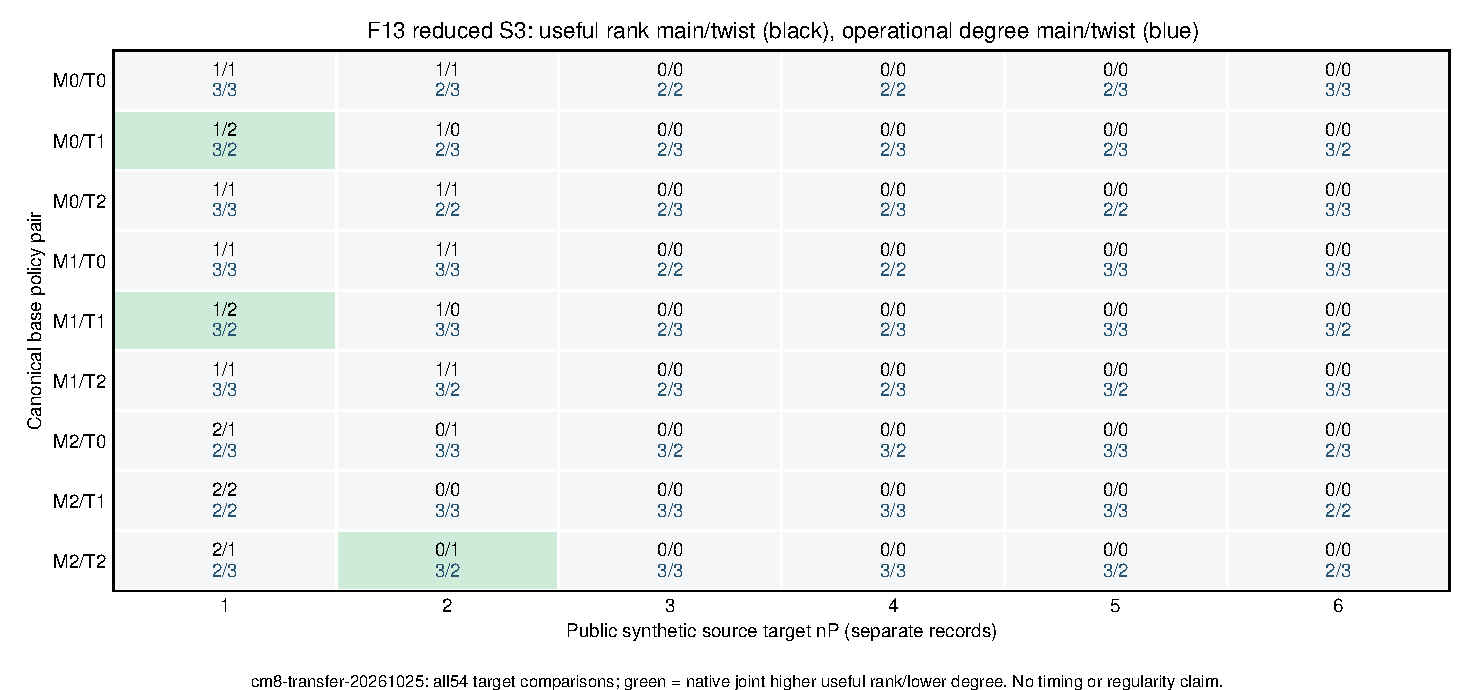
\includegraphics[width=\linewidth]{comparisons.pdf}\end{center}
The graph retains every policy/target. Green identifies exactly the three joint
reduced gains. Each cell shows useful-rank main/twist above operational-degree
main/twist. The strongest source policy is not replaced by a batch average.

Every transported/pulled-back control preserves the ordered accepted lifts,
coefficient rows and useful-rank steps. Of72 matched degree checks,68 equal and
4 differ. At n3,4 main0 to matched0 changes2 to3; twist2 to pullback2 changes3
to2. All four favor the source presentation. Nonlinear encoding changes this
solver degree even when matched relation yield is conserved; the counterevidence
is retained. No uniform twist advantage follows.

\section*{Checked proofs and fail-closed replay}
The unmodified scoped gate passes208 public named theorems/269 audited
declarations, including17 new public theorems/20 declarations; zero failures
or extra trusted axioms. Only propext, Classical.choice and Quot.sound occur.
The new universal cleared Montgomery polynomial has source-bound certificate
IDC1h45f7f67f60c827c3,32+16 native points and false identity/source controls.
It certifies a polynomial only. All16 older identities/sources are unchanged.

Rust independently reproduces field/group arithmetic, roots, incremental
Macaulay rows/promotions, evaluation ranks and full certificates, with a separate
semantic witness audit. It reproduces24 frozen prefix certificates by actual x;
no old scalar labels construct new solver answers. Exact fresh replay and22
backend tests pass. Eleven rehashed controls reject101 without a receipt:
false map/subgroup/source, missing arm/target, degree/witness/row/log/query/scalar.
There are no failed online shifts, so the missing-failed-query control is
explicitly null; missing-query removes a successful query.

Fresh release library4479 tests pass,119 existing ignores; four workflow
metadata tests and naming/card/size/artifact checks are recorded with raw source,
failures and exact commands. Failed Rust borrow/Lean rewrite attempts and an
initial certificate extra-count mismatch remain preserved. No native cap hits.
Native budgets600s, two existing build workers, no paid compute or upload.
Conductor exits127; no task lease or replacement coordinator is claimed.

\section*{Next checkable bridge}
Proposed explicit dual, not tested here: with v=12x-6 on T,
\[
 D_X=10(v+5+8/v)+10,\qquad D_Y=12y(1-8/v^2).
\]
Handle infinity/kernel(7,0), check both compositions equal doubling, then use
$[4]D$ as the order-seven inverse before replacing enumerative base pullback.
Expose source-annihilator hypotheses in a generic group theorem. Preserve all
prior bases/results and price maps separately; no automatic cost gain is implied.
General normalization, geometric maps, broader S3/S4 lifting, stationary useful
yield, generic pairing, trace-zero and calibrated complete work remain open.
No general hardness, speed, GAE/S/rho or external-fastest claim is admitted.
\end{document}
